
\section{Olion paluu 19.--21.4.}

\begin{multicols}{2}

	\noindent Jatkona viime syksyn \textit{Operaatio olio} "=telttaretkelle lippukunnan
	seikkailijavartio \textit{Makkaramokkulat} ja tarpojavartio \textit{Päärynähyttyset} lähtivät
	telttailemaan samoihin Sipoonkorven maastoihin retken jännittävässä jatko"-
	osassa \textit{Olion paluu}, jonka \textit{Vene}"-vartio oli jälleen menestyksekkäästi
	suunnitellut.

	Kaksitoista rusakkoa kokoontui retken lähtöön jo tutussa paikassa,
	Kontulan ostarin Kalkan Pizza"-Kebab"-Grillin edustalla
	perjantai"-iltapäivänä. Kun osa retkeläisistä hyppäsi bussiin kohti
	Viikkiä, osa siirtyi lippukunnan varastolle, jossa logistiikkamestari
	Mikko odotti valmiina hakemaan retken ruoat ja kyyditsemään ne kaluston
	-- ja kantajien -- kanssa telttapaikalle. Bussiosasto jatkoi Viikistä
	Sipoon Myyrakseen. 

	Bussiosastolla oli edessä tuskien taival: 2,4 kilometrin kävely
	pysäkiltä telttapaikan läheiselle parkkipaikalle. Toisaalta, ei
	auto-osastollakaan helppoa ollut kantaa kaikki retken ruoat ja yhteiset
	varusteet parkkipaikalta ylös leiriin. Vaikka matkaa oli vain 700
	metriä, oli leiripaikka viisitoista metriä korkeammalla merenpinnasta
	kuin parkkipaikka. Tehtävästä suoriuduttiin kuitenkin ansiokkaasti.

	Telttapaikalla aloitettiin leirityöt: Osa retkeläisistä alkoi pilkkoa
	puita yötä varten kun taas osa alkoi pystyttää telttaa. Teltan pystytys
	ei sujunut aivan määräajassa, mutta lopputulos oli särmä ja erittäin
	maastokelpoinen -- mitä nyt yhtä kaminan jalkaa etsittiin
	epätoivoisesti, vaikka se oli koko ajan teltan sisällä. Selvästi
	telttaa ei käytetä tarpeeksi, kun kulmasalkojen asentaminen on niin
	paljon voimaa vaativa työ.

	Tässä vaiheessa retkeä alkoi satamaan lunta ja lumentulo jatkuikin aina
	sunnuntaihin asti. Huhtikuista takatalvea ei jääty sen enempää
	ihmettelemään vaan retkeläiset siirtyivät teltan suojaan, jossa kamina
	syttyi melkein itsestään etukäteen valmisteltujen sytykkeiden avulla. 

	\vspace*{0.16cm}
	\noindent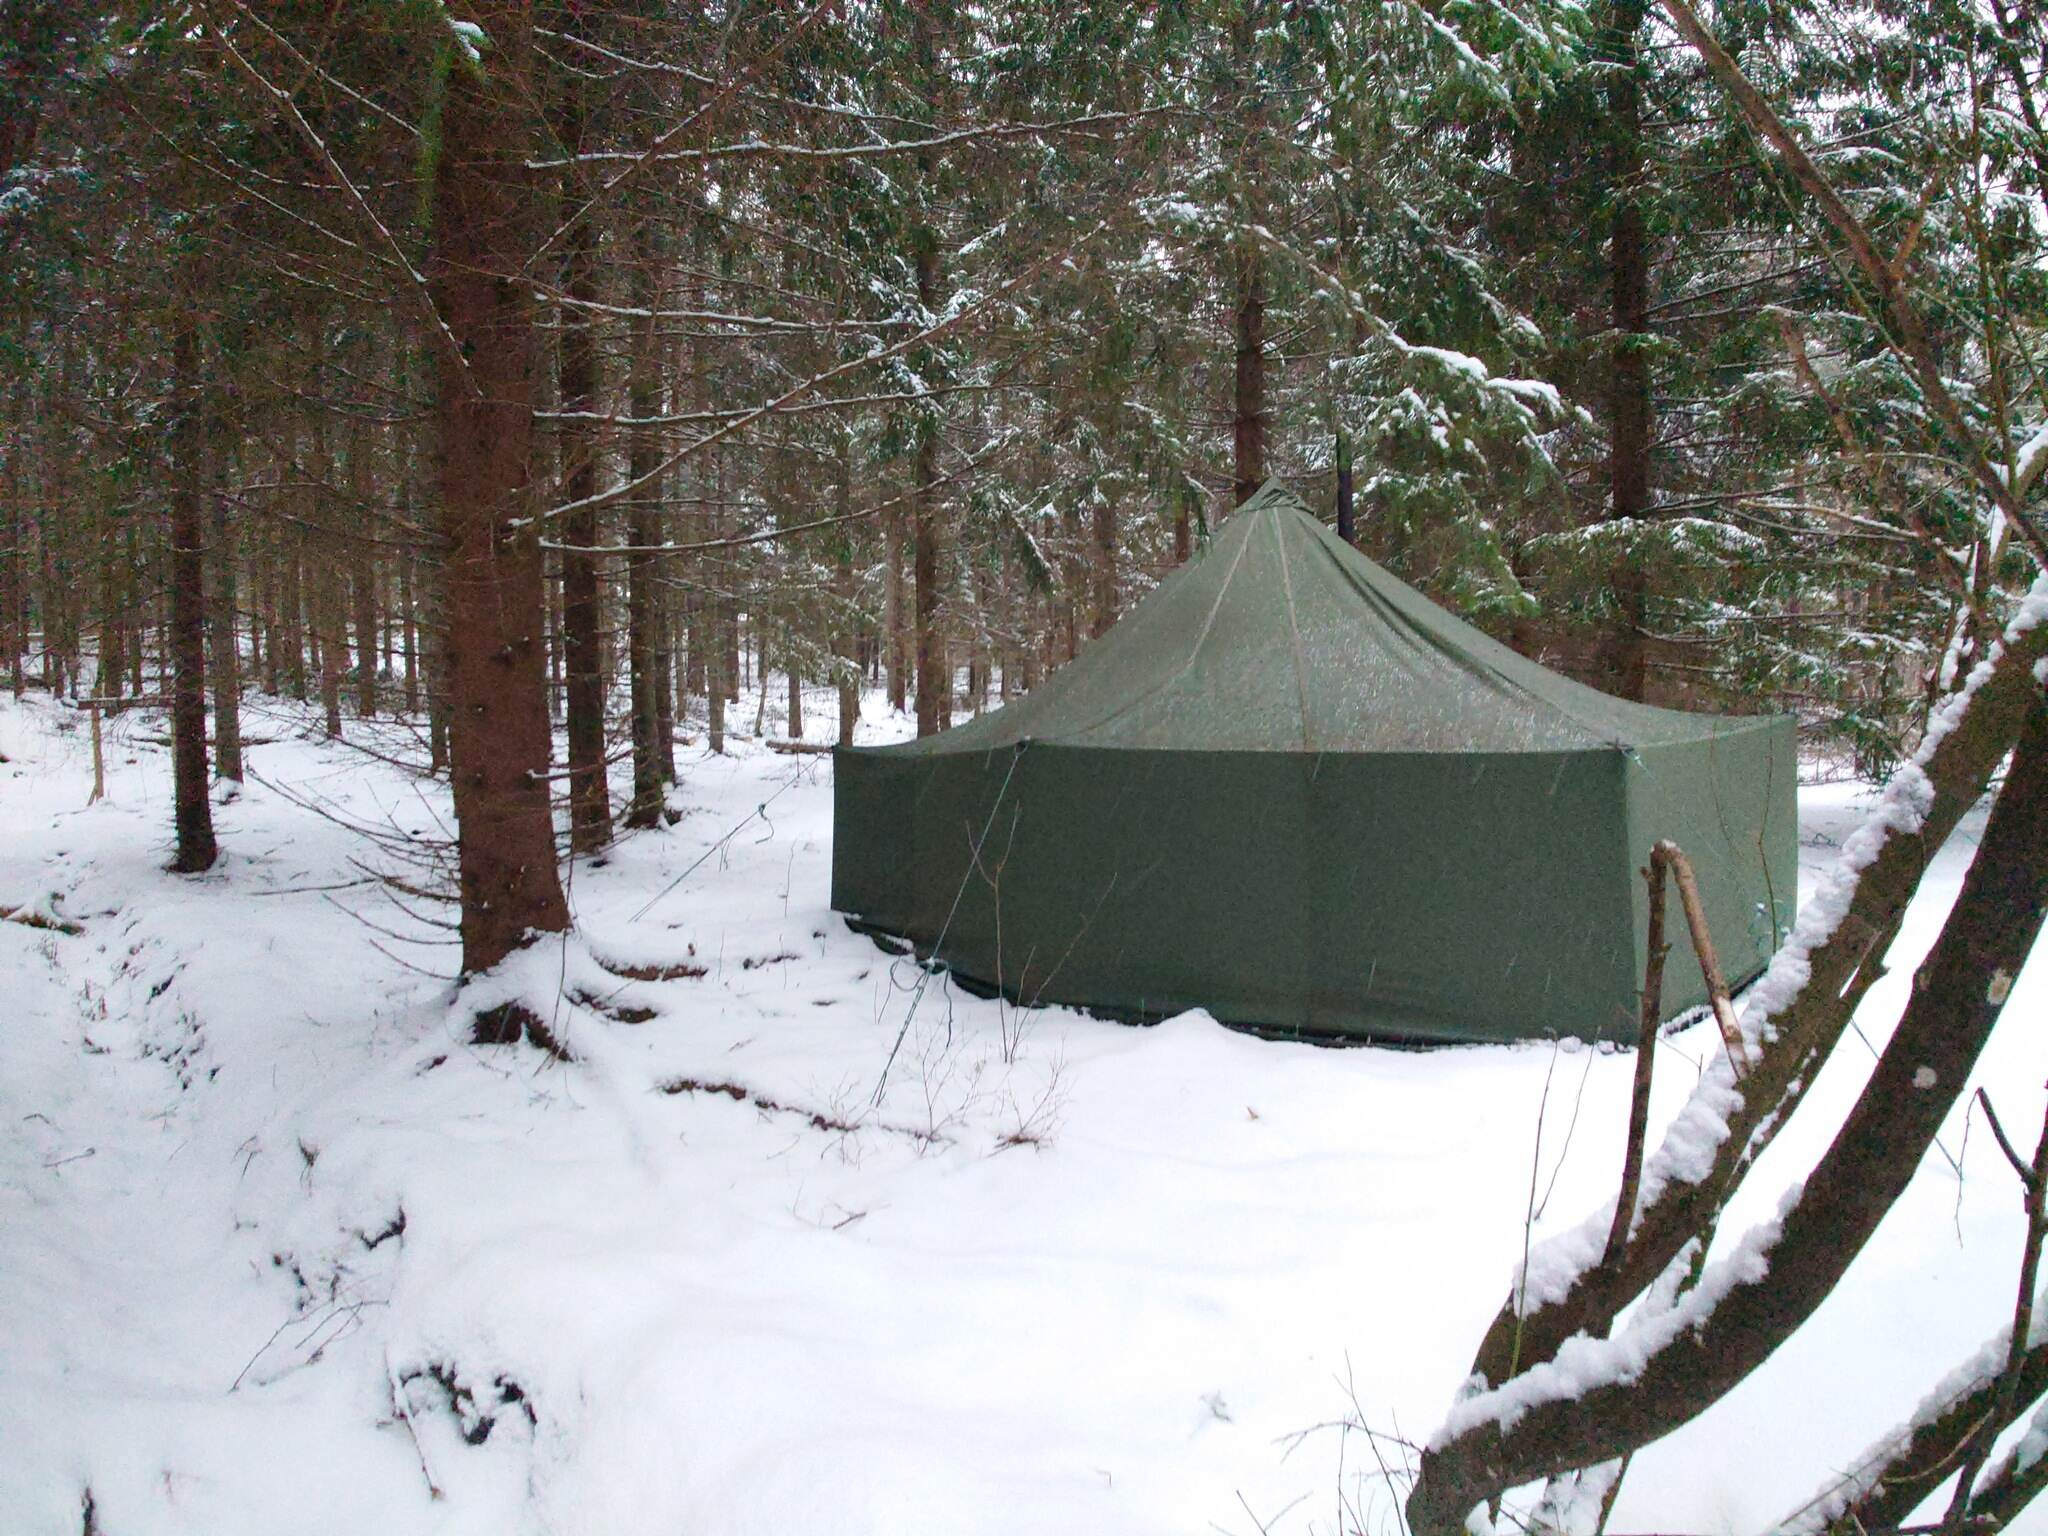
\includegraphics[width=\linewidth]{assets/olionpaluu2}

	Ennen nukkumaanmenoa sovittiin vielä kipinävuoroista: Ensimmäisinä
	kipinävuorossa valvoivat Elias ja Mikael, sitten Alden ja Toivo,
	Joella, Ninni ja Tesla, Ahti ja Kata, Johannes ja Touko, sekä
	viimeisenä Janne. ''Pakastaja Elvi'' ei päässyt yllättämään, vaikka
	kaminaa poltettiinkin säästöliekillä. Ainakin yhden kerran yön aikana
	''lohikäärme'' tuli kuitenkin tarpeeseen, kun kyteville puille piti antaa
	vähän lisäilmaa. Niin ikään osalla retkeläisistä oli aamuksi
	jännitystä, kun Ahti pisti pystyyn F1"-kisastudion.

	\vspace*{0.16cm}
	\noindent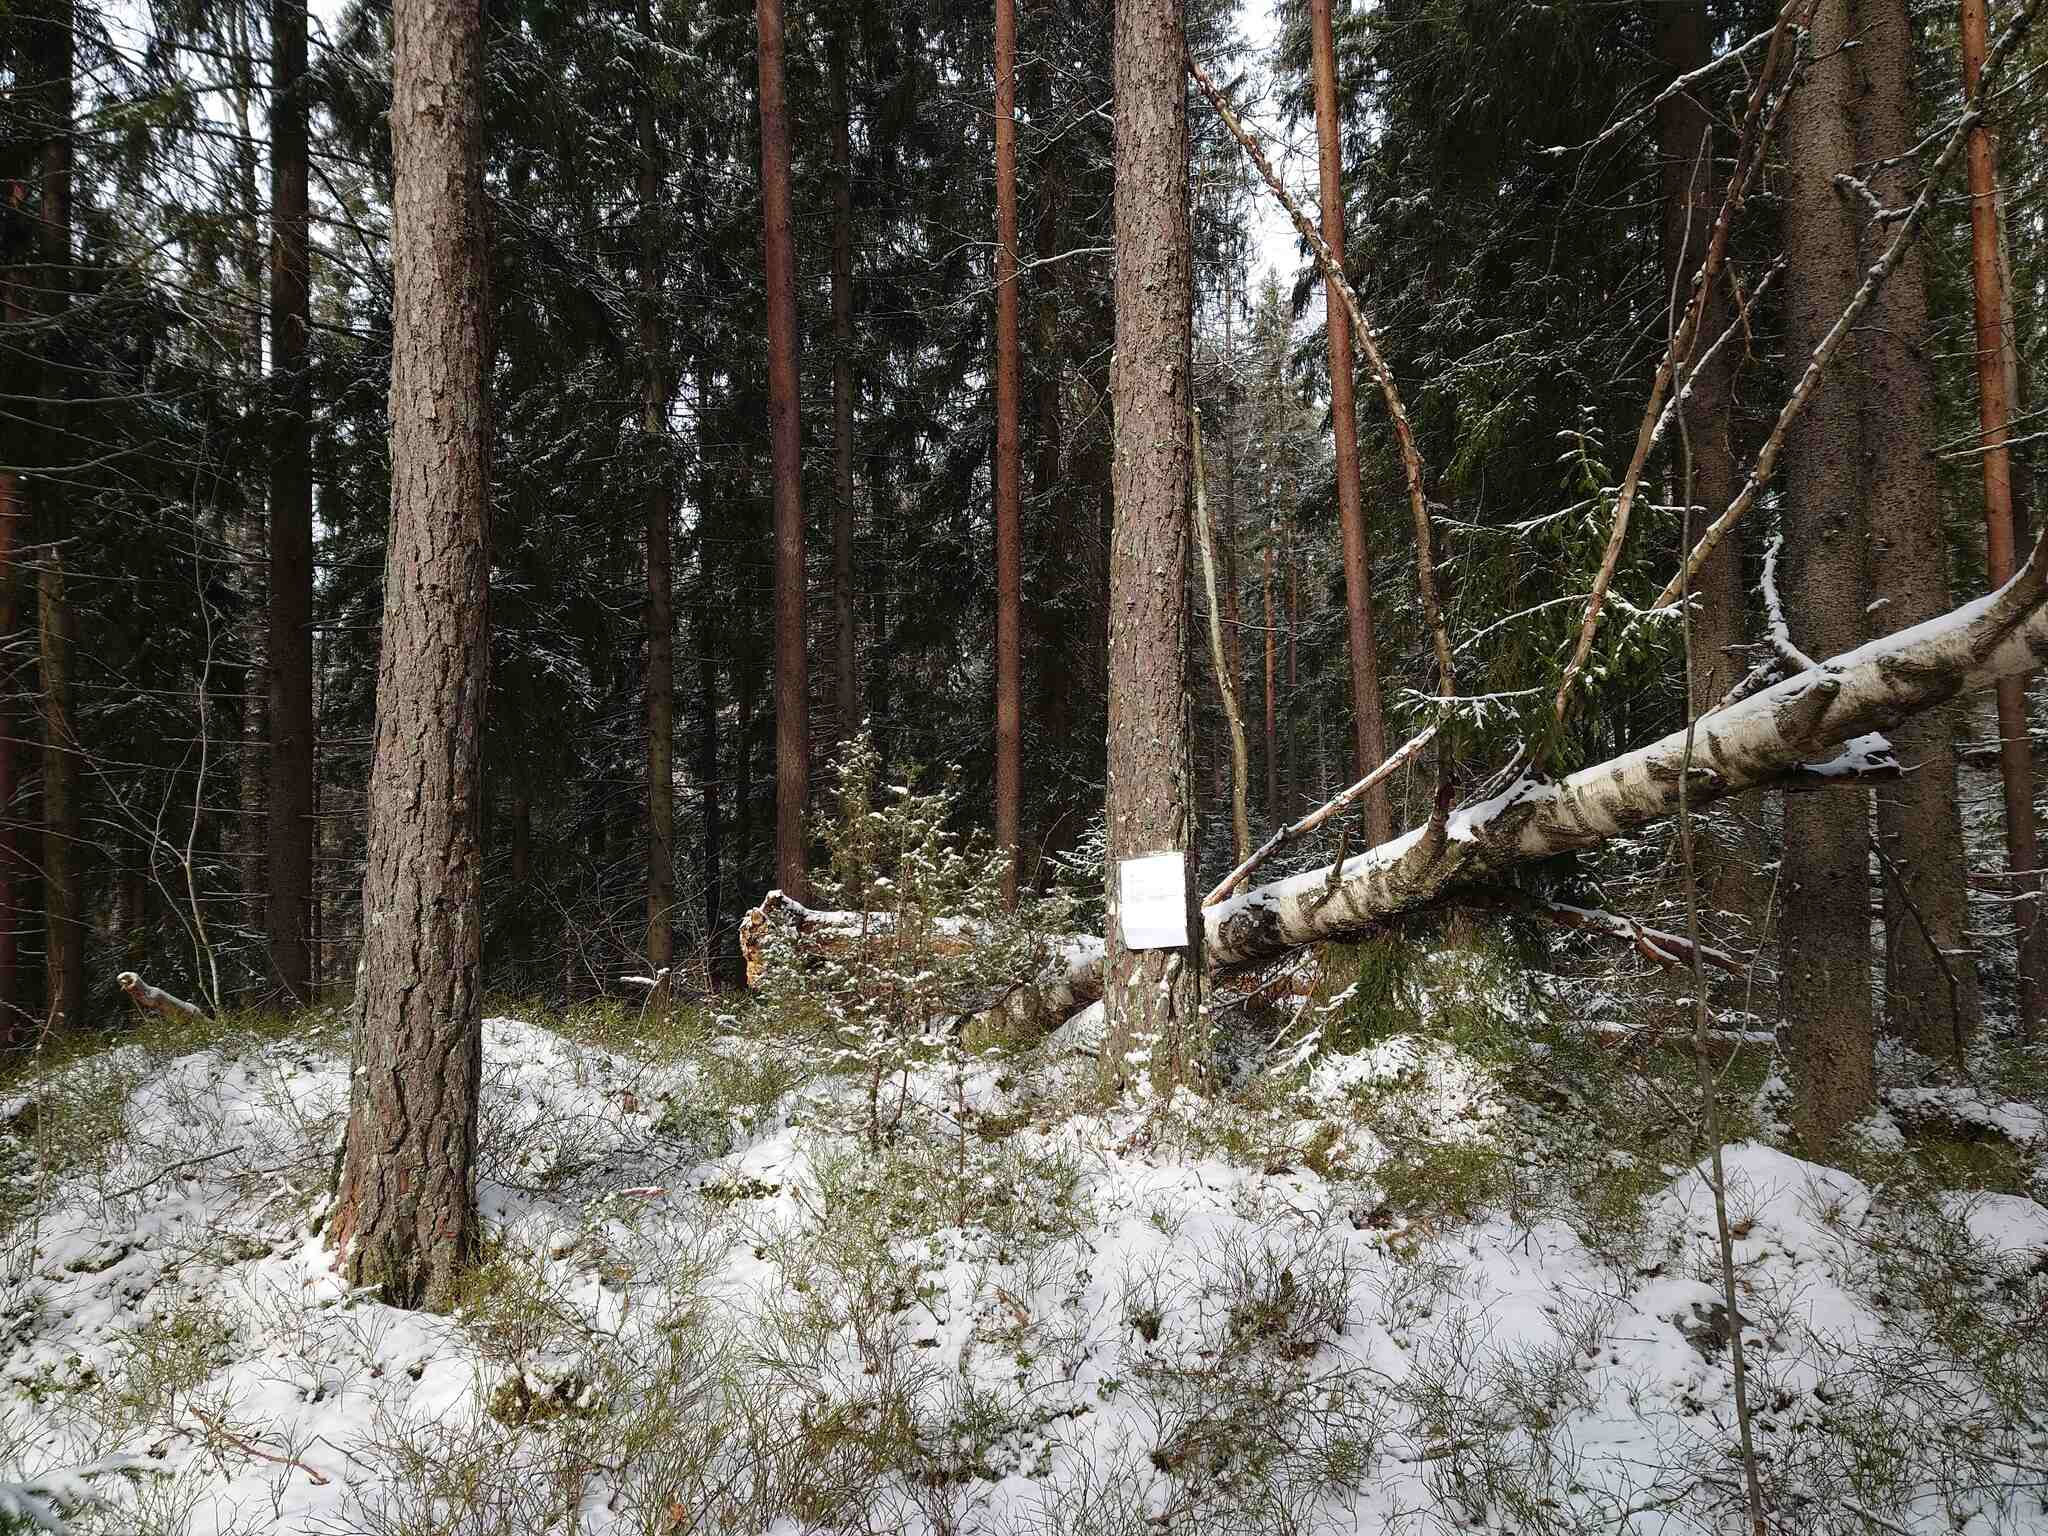
\includegraphics[width=\linewidth]{assets/olionpaluu4}

	Retkeläiset heräsivät valkeaan lauantaiaamuun: lunta oli tullut yön
	aikana useampi sentti ja lämpötila oli muutaman asteen pakkasen
	puolella. Väsyneet ja kohmeiset retkeläiset siirtyivät aamupuuron
	pariin. Ravittuina leikittiin sitten Katan johdolla kaikkien
	suosikkileikkejä kuten pölkkyä ja tervapataa -- jälkimmäistä tosin
	vahvasti kontaktiversiona. 

	Ja taas syötiin: trangioilla valmistui maukasta tonnikalanuudelia ja
	tofunuudelia. Onnistuipa osa retkeläisistä kastelemaan kenkänsä
	nuotiopaikan lätäkössä. Siis vatsat täynnä ja kenkä märkänä aloitettiin
	retken juoneen liittyvä suunnistus. Viiden rastin viuhkasuunnistuksessa
	oli kolme miehitettyä ja kaksi kylmää rastia. Kullakin rastilla
	vartioiden suoritukset pisteytettiin niin käpyjen keräämisessä,
	eläinten jälkien tunnistamisessa, näyttelijän taidoissa, ryhmäkuvan
	ottamisessa kuin laskuvarjon rakentamisessakin. Kultakin rastilta
	selvisi myös vihjeitä salaperäisestä oliosta. 

	Kuten pistetaulukosta voit tarkistaa, pistekilpailun voittajaksi
	selvisi yhden pisteen erolla Minä ja toi "=vartio -- onnittelut!

	Suunnistuksen jälkeen käytiin juoni nopeasti yhdessä läpi ja puolet
	retkeläisistä lähti maitojunalla kotiin. Jäljelle jääneet pilkkoivat
	lisää puita yötä varten ja lämmittivät itselleen kolme kattilallista
	hernekeittoa, joka saatiin melkein kokonaan viiteen pekkaan syötyä!

	\vspace*{0.08cm}
	\noindent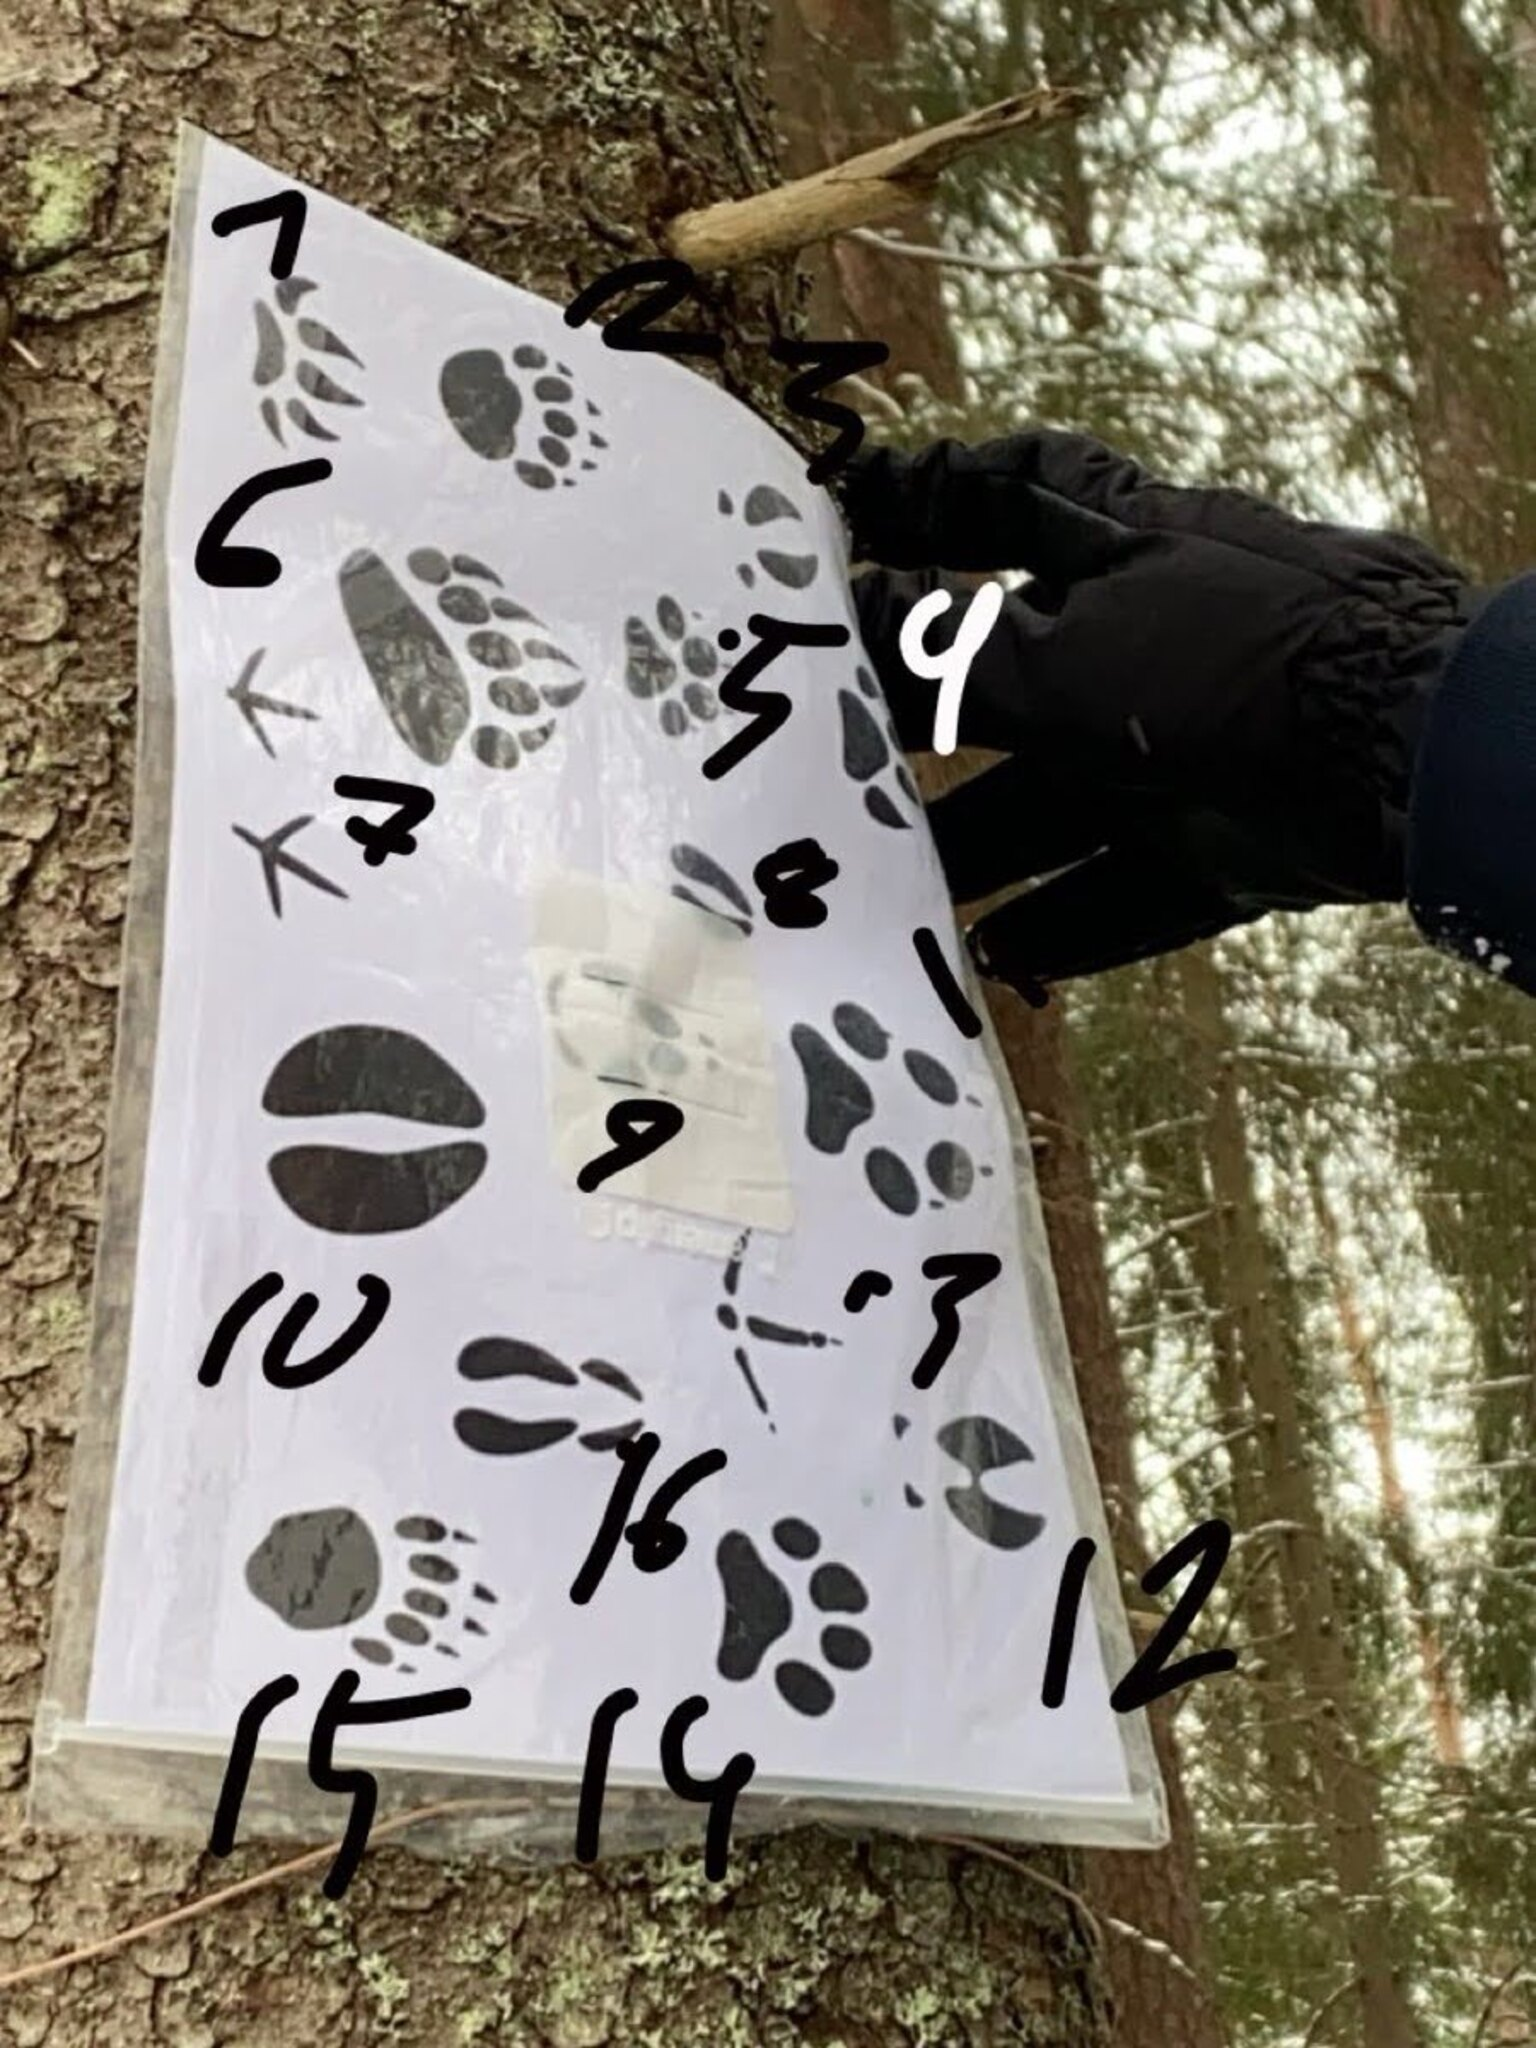
\includegraphics[width=\linewidth]{assets/olionpaluu3}

	Kaikki oli valmista yötä varten. Kello ei ollut vielä kahdeksaakaan,
	mutta retkue päätti siirtyä jo telttaan lämmittelemään ja
	kuivattelemaan varusteita -- ja sivuun telttapaikalle tulleilta muiden
	lippukuntien ryhmänohjaajakoulutettavilta, jotka myös olivat yöpymässä
	puolijoukkueteltalla. Kaminaa poltettiin vähän isommalla liekillä kuin
	ensimmäisenä yönä ja teltan lämmetessä alkoi itse kullakin silmäluomi
	painaa. Kipinävuoroista sovittiin, että ensimmäisenä valvoi Ahti,
	sitten Elias ja viimeisenä Janne. 

	\vspace*{0.08cm}
	\noindent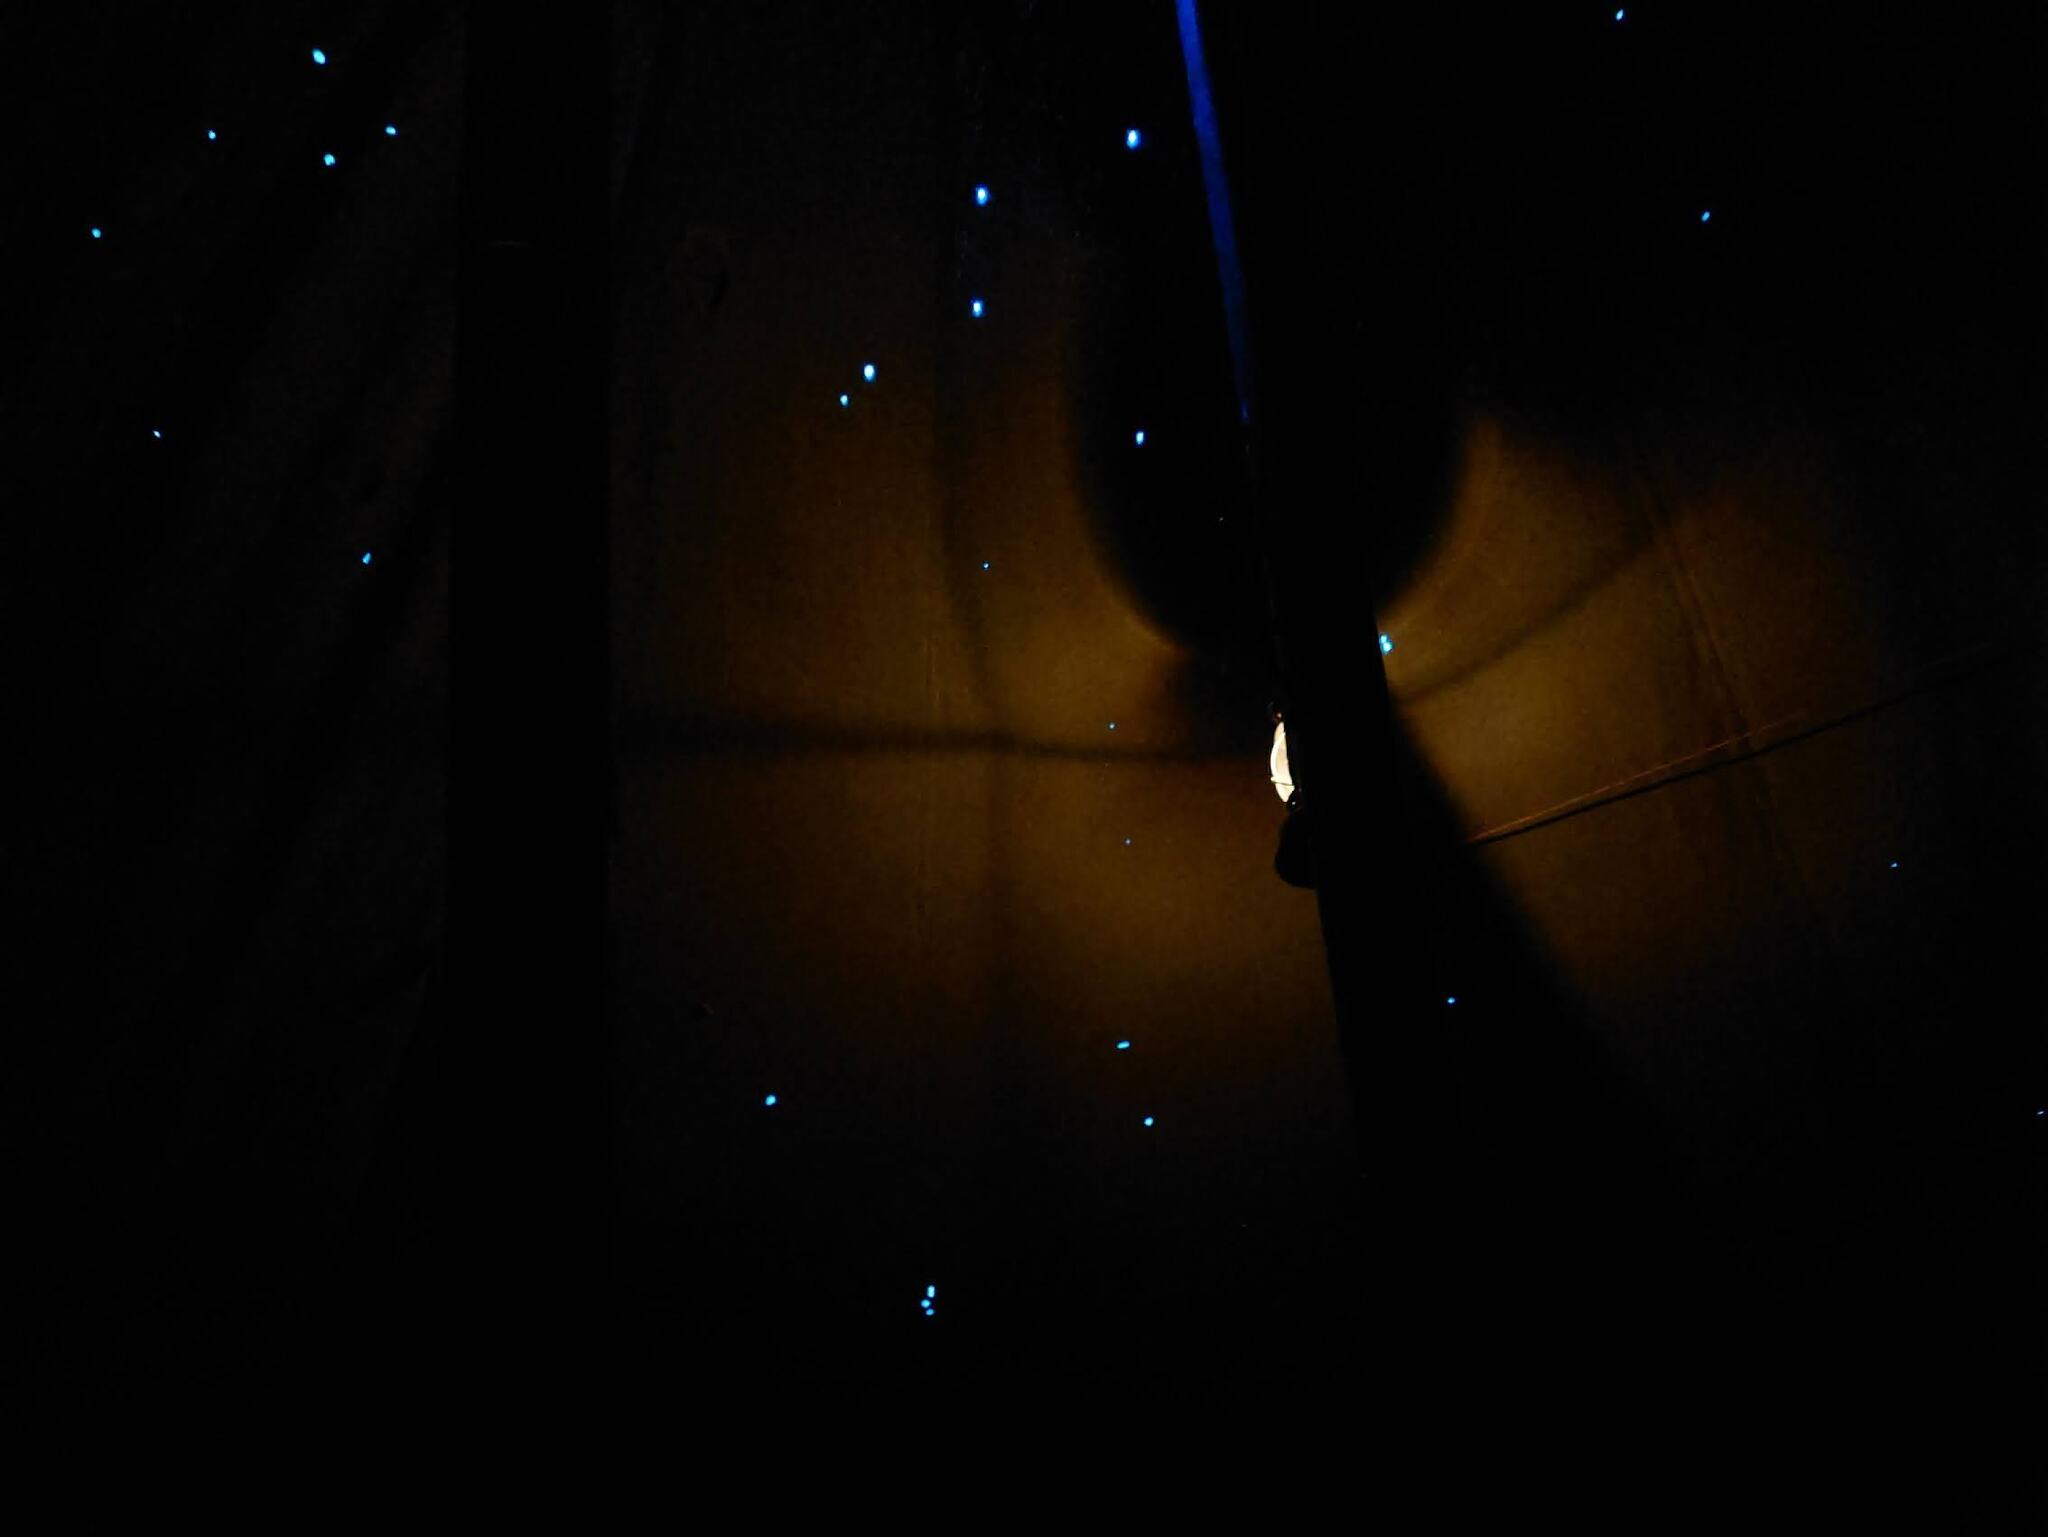
\includegraphics[width=\linewidth]{assets/olionpaluu1}

	Aamu alkoi reippaasti puuroveden kiehuessa kaminan päällä, kun teltan
	sisällä ei ollut tietoakaan ulkoilman kylmyydestä tai kosteudesta.
	Varusteet pakattiin vauhdikkaasti ja teltta pistettiin kasaan. Kaminan
	piippu oli yhdestä kohtaa niin tiukassa, että sen irroittamisessa meni
	tovi. Siitä huolimatta piipun palat saatiin sovitettua siististi
	kaminan sisälle (toim. huom. jotain, jossa allekirjoittanut epäonnistui
	surkeasti varastolla perjantaina).

	Kalustoa alettiin roudata takaisin parkkipaikalle. Alamäkeen kantaminen
	sujui vähän helpommin, mutta märkä teltta oli raskas ja polku paikoin
	liukas. Mikko olikin tullut parahiksi parkkipaikalle vastaan ja auto
	pakattiin kalustolla ja retkeläisillä. Hienosti mahtuivat kaikki mukaan
	ja kotimatka voi alkaa.

	Jää nähtäväksi, palaako olio vielä kolmannen kerran. Joka tapauksessa,
	jos viime syksynä satoi vettä kaatamalla ja nyt keväällä oli takatalvi,
	ei seuraavalle kerralle ole enää kovin montaa sään tuomaa haastetta
	jäljellä!

\end{multicols}

\vspace*{0.64cm}
\makebox[0.94\textwidth][c]{%
	\begin{tabular}{ l p{2cm} |r| r r r r r r }
		&&& \textbf{Rasti 2} & \textbf{Rasti 3} & \textbf{Rasti 4} & \textbf{Rasti 5} & \textbf{Rasti 6} & \textbf{Käytös} \\
		& Maks. & 62 & 10 & 17 & 10 & 10 & 15 \\
		\textbf{Sij.} & \textbf{Vartio} & \textbf{Yht.} \\
		\hline
		\textbf{1} & \textit{Minä ja toi}\newline Johannes ja Tesla & 42 & 10 & 8 & 6 & 7 & 11 & 0 \\
		\hline
		\textbf{2} & \textit{TT}\newline Toivo ja Touko & 41 & 10 & 5 & 8 & 7 & 11 & 0 \\
		\hline
		\textbf{3} & Alden ja Joella & 33 & 4 & 6 & 2 & 9 & 11 & 1 \\
	\end{tabular}%
}

\vspace*{0.64cm}
{\raggedleft Kuvat: Retkeläiset \& Janne Suomalainen\\ Teksti: Janne Suomalainen\\}


